	\newpage
	
\section{PROPOSED SYSTEM}
\subsection{DESCRIPTION}
The game comprises three chapters, each centered around pivotal events, skills, and battles in Arjuna's life. The first chapter serves as a practice level, emulating the training of a young Arjuna in Guru Dronacharya's Gurukul. Our objective for this chapter is to enhance the user's skills, ensuring their qualification to progress to subsequent levels. The levels in this chapter are designed with increasing complexity, gradually acquainting the user with the mechanics and nuances of the game.\\
\\
The second chapter revolves around the legendary account where Arjuna utilizes his skills to protect the vulnerable kingdom of Virata. During their final year of exile, the Pandavas concealed their identities and worked as common laborers in Virata's palace. This chapter not only allows users to demonstrate the skills acquired by completing all levels of the first chapter but also provides a meticulously tailored environment that hones their ability to pinpoint and shoot moving targets. Similar to the Virata battle, which symbolized the uprising and unwavering victory of the Pandavas, this chapter emphasizes the user's agility in dodging occasional arrows shot by adversaries. Failure to evade incoming arrows leads to a reduction in the character's life points, and when these points reach zero, the game concludes. Consequently, this level emphasizes the user's dodging and swerving abilities.\\
\\
The proposed third chapter centers around the climax of the epic Mahabharata i.e. monumental war of "The Mahabharata", for which Arjuna has tirelessly practiced and honed his skills since his early days. This chapter serves as an extraordinary platform for users to showcase their abilities, drawing upon the orientation and practices from the previous chapter. It encompasses precise targeting, shooting, and evasive maneuvers to dodge incoming arrows. Arjuna confronts more formidable adversaries such as Dronacharya, Bhishma Pitamah, Karna, Kripacharya, Ashwathama, and others. Only through complete mastery of accurate targeting, shooting, and dodging skills can victory be assured in this chapter.\\
\\
"The Mahabharata" chapter serves as the culmination of the game, providing a challenging and immersive experience for users to fully demonstrate their prowess. It encapsulates the essence of Arjuna's journey, from his early training to the pinnacle of warfare. As players progress through the game, they acquire skills and knowledge, mirroring Arjuna's own growth and development. By incorporating elements of strategy, precision, and quick reflexes, the game offers an engaging and authentic portrayal of Arjuna's legendary archery prowess. Whether players excel in targeting, shooting, or evading obstacles, their success ultimately hinges on their ability to merge these skills seamlessly. With each chapter building upon the previous one, the game provides a rewarding and immersive experience for players as they embark on a journey inspired by the remarkable life and achievements of Arjuna.


\pagebreak
\subsection{SYSTEM BLOCK DIAGRAM}
\vspace{2cm}
\begin{figure}[h]
	
	\centering
	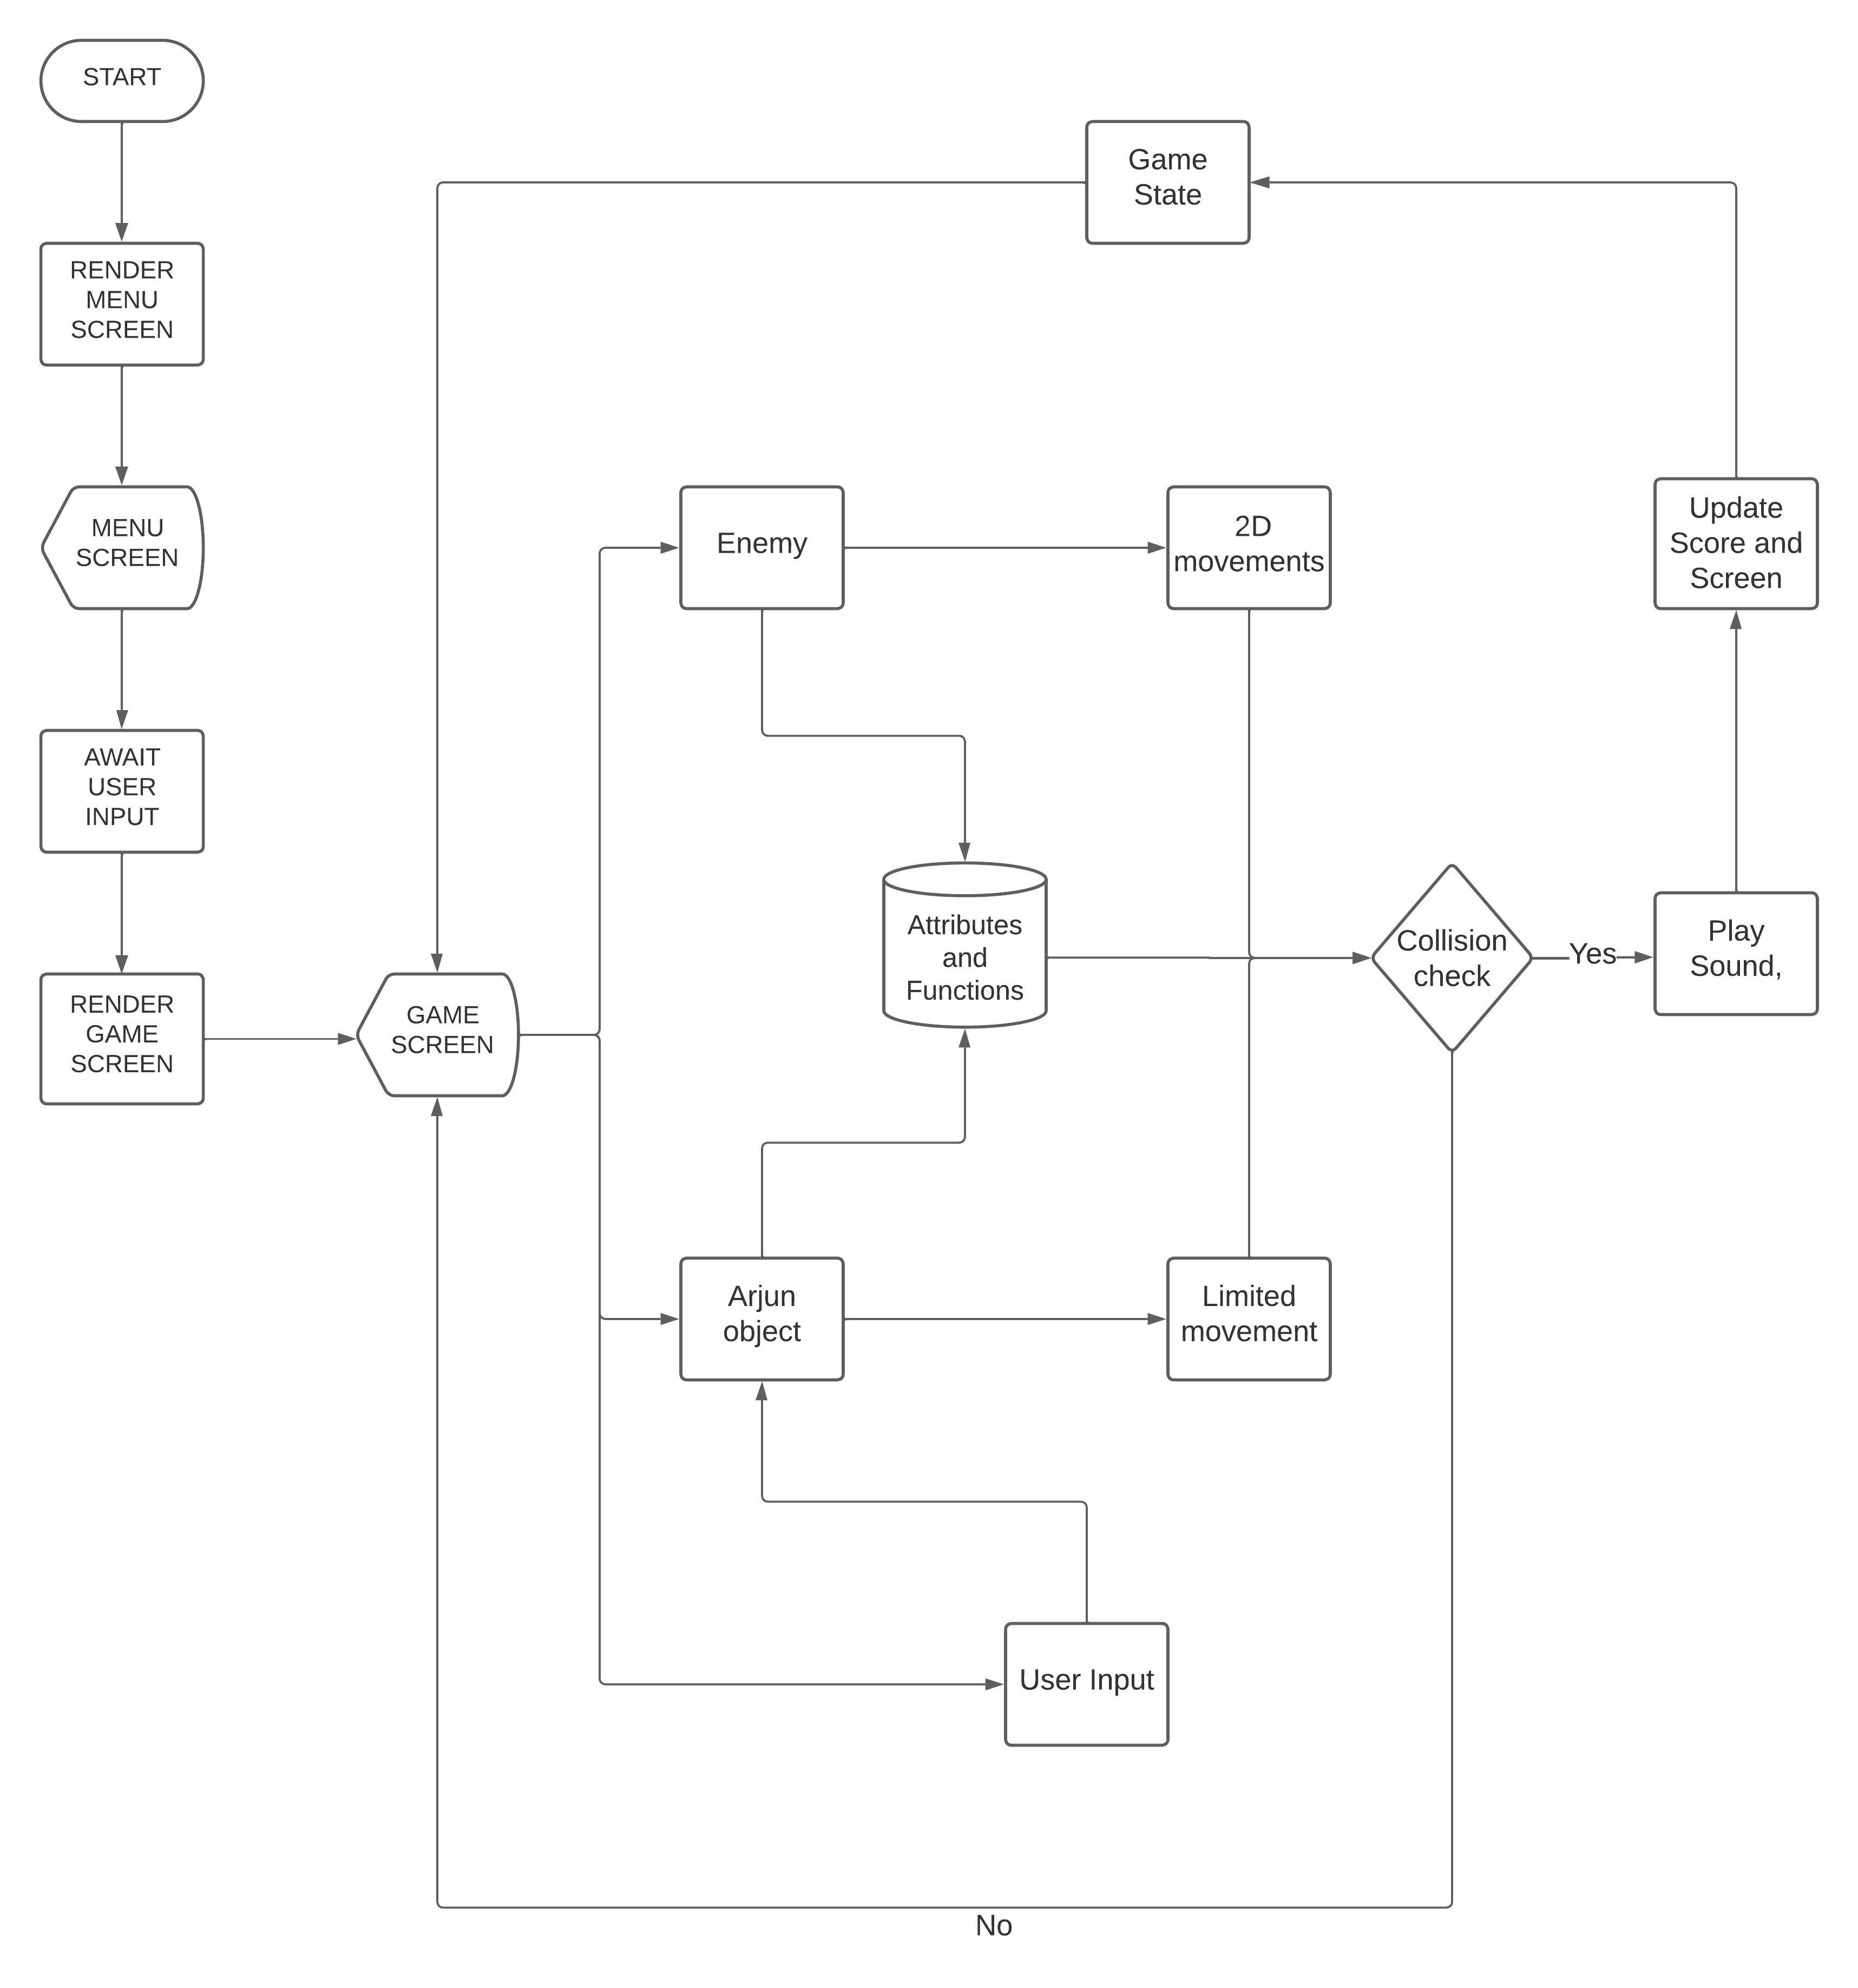
\includegraphics[width = 1.1\textwidth]{sec/pdf/img}

\end{figure}
